\documentclass[a4paper,11pt]{article}
\usepackage[utf8]{inputenc}
\usepackage{geometry}
\usepackage[onehalfspacing]{setspace} 
\usepackage{graphicx}
\usepackage{tabularx}
\usepackage[hidelinks]{hyperref}
\usepackage{float} 
\usepackage{ragged2e}
\usepackage{biblatex} 
\usepackage{listings}
\usepackage{xcolor}


\lstset{
  basicstyle=\ttfamily\footnotesize, % Typewriter font
  keywordstyle=\color{blue},         % Keywords in blue
  commentstyle=\color{gray},         % Comments in gray
  stringstyle=\color{red},           % Strings in red
  breaklines=true,                    % Wrap long lines
  numbers=left,                       % Line numbers on the left
  numberstyle=\tiny\color{gray},      % Line number styling
  frame=single,                       % Box around code
}

\addbibresource{literatur.bib}
\setlength{\bibitemsep}{1em}
\setlength{\arrayrulewidth}{0.3mm}
\setlength{\tabcolsep}{8pt}

\title{Chat Application Project Report}
\author{Hussein Hafid, Jan Rahimi, Mohamad Alzein, Zakaria Abdulkadir}
\date{March 6, 2025}

\begin{document}
\justifying
\pagenumbering{arabic}

\maketitle

\section*{Course}
Object-Oriented Applications (DAT055)

\section*{Repository Link}
\url{https://github.com/Zakoroo/Project-Group-6.git}
\newpage

\section*{Abstract}
This project was developed as part of the Object-Oriented Programming course at Chalmers University, focusing on designing and implementing a chat application. The project followed an object-oriented approach, utilizing UML design, CRC cards, and separate UML diagrams for both the client and server to structure the system effectively. The application was developed using JavaFX for the user interface and Maven for dependency management and logging.
The chat application allows users to create and join chat rooms and send both text and image messages. After implementation, the application was tested and successfully met the minimum project requirements. Despite the challenges of working with JavaFX, which was new to all team members, the team adapted and built a well-structured foundation that allows for future development. Potential improvements include real-time updates, enhanced user authentication, database integration for message history, and better scalability.
This project not only strengthened our technical skills in Java and object-oriented programming but also improved our teamwork and problem-solving abilities, making it a valuable learning experience.



\newpage
\tableofcontents
\newpage
\listoffigures
\newpage
\listoftables
\newpage


\section{Introduction}
This report presents the development of a software project undertaken as part
of the Object-Oriented Application Development course at Chalmers University of
Technology. Over a period of eight weeks, our team of four students
collaborated to design and implement a structured and scalable application,
applying key principles of object-oriented programming and software
engineering. The project provided an opportunity to deepen our understanding of
system architecture, design patterns, and collaborative software development.
This report documents the development process, the technologies utilized, and
the overall experience of working as a team in a structured software project.

\subsection{Project Requirements}
The chat application is designed to provide users with a seamless and
interactive messaging experience. Users can easily connect to a chat, ensuring
real-time communication with others. A persistent chat history is maintained,
allowing users to access past conversations whenever needed. The application
supports sending both text messages and images, enabling rich and dynamic
interactions. Additionally, users can receive new messages or images instantly
when sent by others, ensuring smooth and continuous communication. Each message
or image clearly displays the sender’s identity, allowing users to track
conversations effectively. These features work together to create an efficient
and user-friendly chat system.

\subsection{Scope of the Application}
[placeholder text]

\subsection{CRC Cards}
CRC (Class-Responsibility-Collaboration) cards are used in software design to
identify and define the key classes in a system, along with their
responsibilities and interactions. They help in breaking down the system into
manageable components by specifying what each class does and how it
collaborates with others. In this chat application, the identified classes
include User, Chat (room), and Message, with key responsibilities such as
viewing chat history, sending text messages and images, and receiving new
messages. However, additional classes are needed to manage server-client
communication and database interactions. CRC cards aid in structuring the
system effectively, ensuring clarity in design and functionality distribution.

% CRC cards start %
\begin{table}[h!]
    \centering
    \begin{tabular}{ |p{6cm}||p{6cm}|  }
        \hline
        \multicolumn{2}{|c|}{Class: Chat room}   \\
        \hline
        Responsibility         & Collaborators   \\
        \hline
        1. Manage chat members & User            \\
        2. Store chat history  & Message         \\
                               & Message handler \\
                               & Chat server     \\
        \hline
    \end{tabular}
    
\end{table}
\begin{figure}[h]\centering\caption{CRC Cards for Chat room and Message
    }\label{CRC cards}\end{figure}
% CRC cards end   %

Figure \ref{CRC cards} shows the CRC cards for the Chat Room and Message classes in the chat application. The Chat Room class is responsible for managing room members and storing chat history. It collaborates with the User class to handle room members and interacts with the Message, Message Handler, and Server to maintain the chat history. The Message class is responsible for managing message information and collaborates with both the User and Chat Room classes to ensure proper message handling within the application.

\section{Design of the Chat Application}
The development of our chat application follows a structured and iterative
approach, ensuring flexibility and continuous improvements throughout the
project. We began with an idea-storming phase, where we explored various
features, user needs, and technical requirements. This brainstorming session
helped us lay a strong foundation for the application's design and
functionality.

To maintain a clear and systematic development process, we employed Unified
Modeling Language (UML) to create both a scenario model and a design model. The
scenario model helped us visualize different user interactions and workflows
within the application, while the design model provided a structured blueprint
for the system architecture. These models serve as a guiding framework,
ensuring that all components of the application are well-structured and
logically connected.

For the development, we chose Java as the primary programming language due to
its robustness, cross-platform compatibility, and extensive support for
network-based applications. Additionally, we utilized SQL for database
management to handle user data, messages, and other relevant information
efficiently. This combination of technologies ensures that our chat application
is both scalable and secure.

\subsection{Overview of Software Architecture}
When it comes to designing a chat application one of the important things to
consider is identifying the needs, delegating responsibilities and ensuring data
integrity along the process of transferring information between sever and
client. For instance how are we going to make sure a client cannot send
messages to chat room they are not a member to? How are we going to disallow
tampering with user information? Who is responsible for informing the user of
new messages arriving at certain chat room? These are questions that must be
addressed as early as possible during the design phase to allow seamless
workflow during the implementation phase. 

The first design decision we had to make is to determine how we can store data
including user information, chat rooms and chat log. The idea we agreed upon 
eventually was use a SQL database to store all data. But the question was how are
we going to send information to the database. Are we going to allow the user application
to interact immediately with a database or is there going to be an application on 
the server which hosts the database that define the protocols of interaction and 
data transfer? There were two main problems with allowing immediate

\subsection{Server-Side Design}
\subsubsection{Data Storage and Management}
\subsubsection{Server TCP Communication}
\subsection{Client-Side Design}
\subsubsection{Client Authentication}
\subsubsection{Client TCP Communication}
\subsubsection{Client Interaction and User Interface}
\subsection{Class Design with CRC Cards}
\section{Implementation and design improvements}
\subsection{Workflow}
\subsection{Server application}

\subsection{Client application}
\section{Running the Application}
\subsection{System Requirements}
\subsection{Prerequisites}
\subsection{Installation}
\subsection{Usage}
\subsubsection{User Login}
\subsubsection{User Registration}
\subsubsection{The Main View}
\subsubsection{Searching for Chat Rooms}
\subsubsection{Joining Chat Rooms}
\subsubsection{Connecting to Chat Rooms}
\subsubsection{Sending and Receiving Messages}

\section{Discussion}
\subsection{Development Workflow}
\subsection{Challenges and Difficulties}
\subsection{Limitations}
\subsection{Conclusion}
\subsection{Future Improvements and Enhancements}

\newpage
\section{Sample Code}
\lstinputlisting[language=Java, caption=Example Code]{sample.txt}
\begin{figure}[h]\centering\caption{Java Code Example - Chat Client}\end{figure}

\newpage
\section{Sample UML Diagram}
\begin{figure}[h]
    \centering
    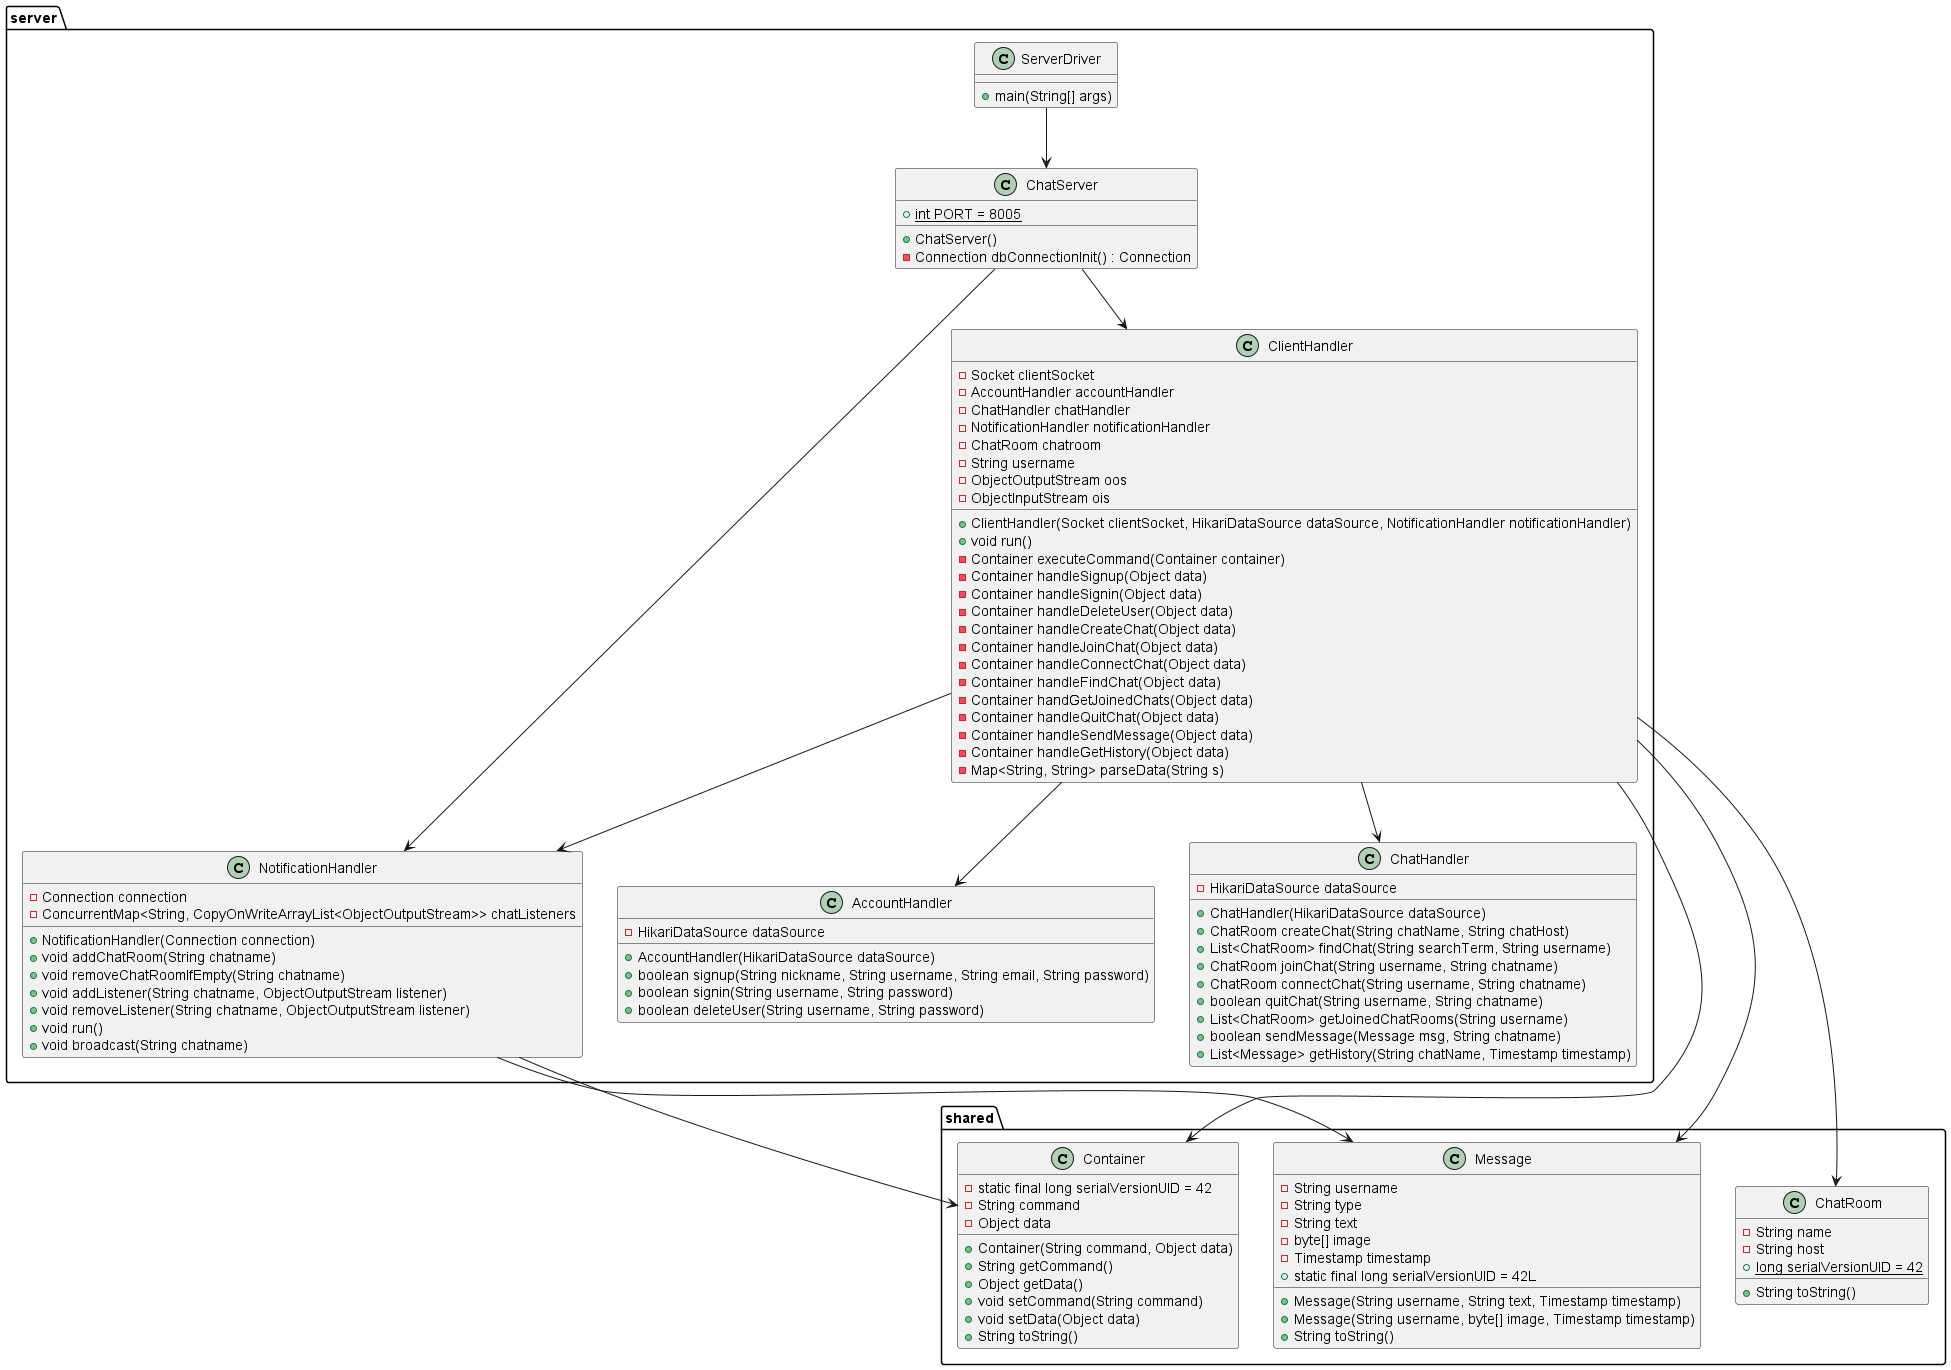
\includegraphics[width=0.8\textwidth]{server.png} % Change to your actual UML diagram file
    \caption{UML Diagram - Chat Client}
\end{figure}

\newpage
\pagenumbering{Roman}
\setcounter{page}{5}
\renewcommand\refname{References}
\addcontentsline{toc}{section}{References}
\printbibliography

\end{document}
